\begin{frame}
  \frametitle{k-Nearest Neighbors}
  \begin{adjustwidth}{-10pt}{0pt}
  \begin{minipage}{0.5\textwidth}
    Objective: \\
    Minimum distance between test sample and training instance(s) \\
    %$$ Y(\boldsymbol{X}) = \frac{1}{k} \sum_{x_i \in N_k(\boldsymbol{X})} y_i $$
    \\~\\
    Algorithm hyperparameters:
    \begin{itemize}
      \item k \textit{(2-5)}
      \item Distance measure \textit{(Manhattan distance)}
      \item Weight of nearest neighbors: uniform or distance \textit{(distance)}
    \end{itemize}
  \end{minipage}%
  \hfill
  \begin{minipage}{0.5\textwidth}
    \begin{figure}
      \centering
      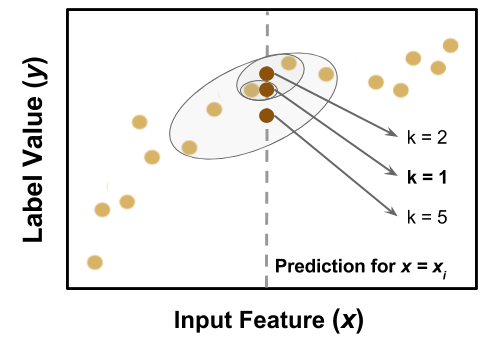
\includegraphics[height=0.5\textheight]{./figures/nn-fig.png}
      \caption{Demonstration of the prediction variation of kNN with different values of \textit{k}}
    \end{figure}
  \end{minipage}
  \end{adjustwidth}
\end{frame}

\begin{frame}
  \frametitle{Decision Trees}
  \begin{adjustwidth}{-15pt}{0pt}
  \begin{minipage}{0.63\textwidth}
    \begin{figure}
      \centering
      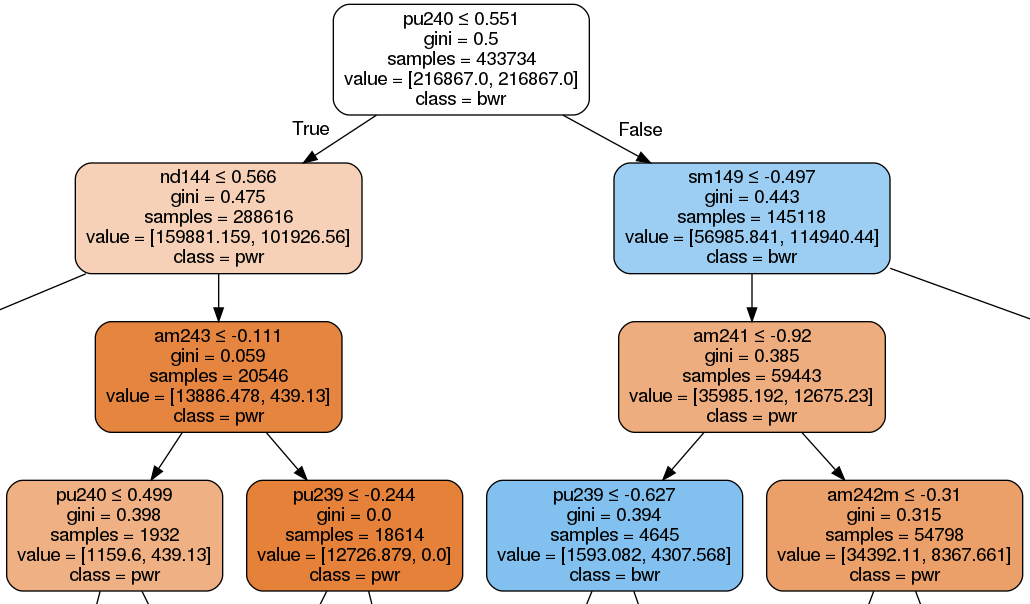
\includegraphics[width=\textwidth]{./figures/dtree_crop.png}
      \caption{Cropped image of a decision tree of reactor type prediction}
    \end{figure}
  \end{minipage}%
  \hfill
  \begin{minipage}{0.4\textwidth}
    Objectives: %maximize information gain for each split or minimize \\
    \begin{itemize}
      \item Classification: information gain
      \item Regression: mean error
    \end{itemize}
    Algorithm hyperparameters:
    \begin{itemize}
      \item Maximum \# of features \textit{(num nuclides, or None)}
      \item Maximum depth \textit{(varies, or None)}
      \item Criterion \textit{(Scikit defaults: gini \& mean squared error)}
    \end{itemize}
  \end{minipage}
  \end{adjustwidth}
\end{frame}

\begin{frame}
  \frametitle{Maximum Likelihood Calculations}

Likelihood calculated is as follows:
\[L(M|r_{test}) = \prod_i \frac{1}{\sigma_{i,sim} \sqrt{2\pi}} \exp{\frac{-(r_{i,test} - r_{i,sim})^2}{2 \sigma_{i,sim}^2}}\]

Whereas the log-likelihood is used in practice:
\[ln(L(M|r_{test})) = \sum_i ln(\frac{1}{\sigma_{i,sim} \sqrt{2\pi}}) - \frac{(r_{i,test} - r_{i,sim})^2}{2 \sigma_{i,sim}^2}\]

Approach based on previous work: \cite{mll_method, mll_sensitivity} \\~\\

\end{frame}
